\documentclass{article}

\usepackage{arxiv}

\usepackage[utf8]{inputenc} % allow utf-8 input
\usepackage[T1]{fontenc}    % use 8-bit T1 fonts
\usepackage{setspace}
\setstretch{1.2}          % improved readability (line spacing)

\usepackage{hyperref}       % hyperlinks
\usepackage{url}            % simple URL typesetting
\usepackage{booktabs}       % professional-quality tables
\usepackage{amsfonts}       % blackboard math symbols
\usepackage{amsmath,amssymb}
\usepackage{nicefrac}       % compact symbols for 1/2, etc.
\usepackage{microtype}      % microtypography
\usepackage{graphicx}
\usepackage{float}
\graphicspath{ {./images/} }
\AtBeginDocument{
  \newgeometry{
    textheight=9in,
    textwidth=5.1in,
    top=1in,
    headheight=14pt,
    headsep=25pt,
    footskip=30pt
  }
}
\raggedbottom
\providecommand{\tightlist}{%
  \setlength{\itemsep}{0pt}\setlength{\parskip}{0pt}}

\title{TinyCortex (Draft)\\\large Building Artificial Consciousness with a High-Throughput Context System}

\author{
  Tiny Humans \\
  \texttt{research@tinyhumans.ai} \\
}

\begin{document}
\maketitle
\begin{abstract}
\vspace{-0.2em}
{\small
\begin{minipage}{\linewidth}
\setlength{\parskip}{0.35em}
\noindent
Large language models are good at short tasks, but they still struggle with
long-term coherence and adaptation. Most systems retrieve information, answer,
and move on.

\smallskip\noindent
We present \textbf{TinyCortex}, a simple ongoing intelligence loop built on top
of memory. The loop continuously processes experience, learns from feedback,
forgets low-value noise, and updates a persistent internal state over time.
\smallskip\noindent
TinyCortex has two components: \textbf{(1)} a memory layer and
\textbf{(2)} a consciousness loop. Together they provide persistent context
and continuous adaptation.

\smallskip\noindent
\textbf{Current result.} In internal usage, this approach improves continuity
across sessions and helps the system adapt faster to a user's evolving context.
Our claim is practical: stronger feedback, learning, and forgetting dynamics
can move AI systems closer to consciousness-like behavior and, over time, to
AGI-level adaptability.
\end{minipage}
}

\end{abstract}
% \vspace{-0.5em}

% Start the body on a fresh page so the first long paragraph is not split
% awkwardly under the figure (avoids mid-sentence page breaks at the header).
% \clearpage

\section{Introduction}

Modern LLMs are strong at local reasoning but weak at long-horizon
coherence. Three constraints repeatedly appear in production systems:
\textbf{(i)} finite context windows, \textbf{(ii)} retrieval pollution in
RAG-style pipelines (irrelevant or stale evidence), and
\textbf{(iii)} lack of instinct-like consciousness, which keeps behavior
narrow and reactive. Increasing context length helps only partially, because
cost scales with sequence length and quality often drops when the active prompt
carries too much low-signal text.

This shifts the design focus from ``more context'' to ``better memory
control.'' Practical systems must decide which evidence to admit, which
evidence to decay, and which state transitions to preserve as durable
history.

TinyCortex is explicitly two things: a memory layer and a consciousness loop.
The memory layer provides durable context; the consciousness loop provides
continuous adaptation through feedback, learning, and forgetting. Together,
they transform stored context into evolving intelligence.

Human memory provides a useful engineering analogy. Biological systems handle
continuous noisy input through selective gating, reinforcement by use, and
time-based forgetting. Most current LLM memory stacks implement storage and
retrieval well, but still under-specify these three control functions:
\textbf{what to keep}, \textbf{what to strengthen}, and
\textbf{what to update over time}.

We introduce \textbf{TinyCortex}, an architecture for conscious
intelligence designed around those control functions. It combines:
\begin{itemize}
\item Semantic and graph retrieval for topical and relational recall;
\item An ordered state-event ledger for deterministic temporal/state queries;
\item Retention-aware reweighting and decay to suppress memory pollution;
\item Interval-based thought synthesis to maintain latent internal state
between explicit prompts.
\end{itemize}

Figure~\ref{fig:consciousness-architecture} summarizes the architecture.
Our central claim is operational: consciousness-like continuity requires both
an adaptive memory substrate and a recurrent intelligence loop. The memory
layer and the consciousness loop work together to produce adaptation over time.

\section{Related Work}

\subsection{Titans and MIRAS: Long-Term Memory for Language Models}

Google's Titans line reframes sequence modeling by separating fast
in-context processing from a slower persistent memory path
\cite{behrouz2025titans}. Instead of relying only on larger context windows,
Titans introduces a learned long-term mechanism that complements attention on
long horizons.

The MIRAS perspective extends this idea by treating sequence models as
associative memory systems with explicit retention and biasing dynamics
\cite{behrouz2025allconnected}. Retrieval and retention are first-class
inference-time mechanisms rather than side effects of attention alone.

These directions are promising but remain mostly research-stage.

\subsection{GraphRAG and Graph-Based Memory and Retrieval}

GraphRAG demonstrates that graph structure can improve retrieval beyond flat
vector similarity by enabling entity-centric and global reasoning over
corpora \cite{edge2024graphrag,microsoft2025graphragdocs}. A recurring
tradeoff is ingestion overhead: high-quality graph extraction and linking can
be expensive and slow at large scale.

\subsection{MemoryBank: Retention-Aware Memory for Language Models}

MemoryBank \cite{zhong2023memorybank} is a direct precursor to
retention-aware LLM memory. It models memory strength over time and updates
retention from interaction signals, rather than treating memory as static
retrieved text.

\section{Understanding the Human Brain}

Before implementation details, we ground the design in biological principles.
The goal is not neural equivalence, but transferable mechanisms for memory
selection, retention, and consolidation.

\subsection{Purkinje Cells}
\textit{The ``we problem''} in artificial consciousness can be framed as
coordination: how distributed signals become a coherent self-model that acts
as a unified agent. In biology, this coherence emerges from layered circuits,
not a single unit.

Purkinje cells offer a useful analogy for combining \textit{background
activity} with \textit{coordinated control}. They integrate high-dimensional
parallel input while maintaining ongoing, partly stochastic firing. This
endogenous activity supports fine timing and internal adjustment, not only
stimulus-response reactivity.

For memory systems that treat ambient \emph{noise} and \emph{conscious
thoughts} as first-class signals (Figure~\ref{fig:consciousness-architecture}),
the key lesson is permission for controlled spontaneous initiation.
Internally generated candidates can surface and then be amplified or
suppressed through feedback. Three principles carry over:
\textbf{(i)} high-dimensional integration,
\textbf{(ii)} time-varying endogenous candidate generation, and
\textbf{(iii)} selective inhibitory gating calibrated by interaction.

\begin{figure}[H]
\centering
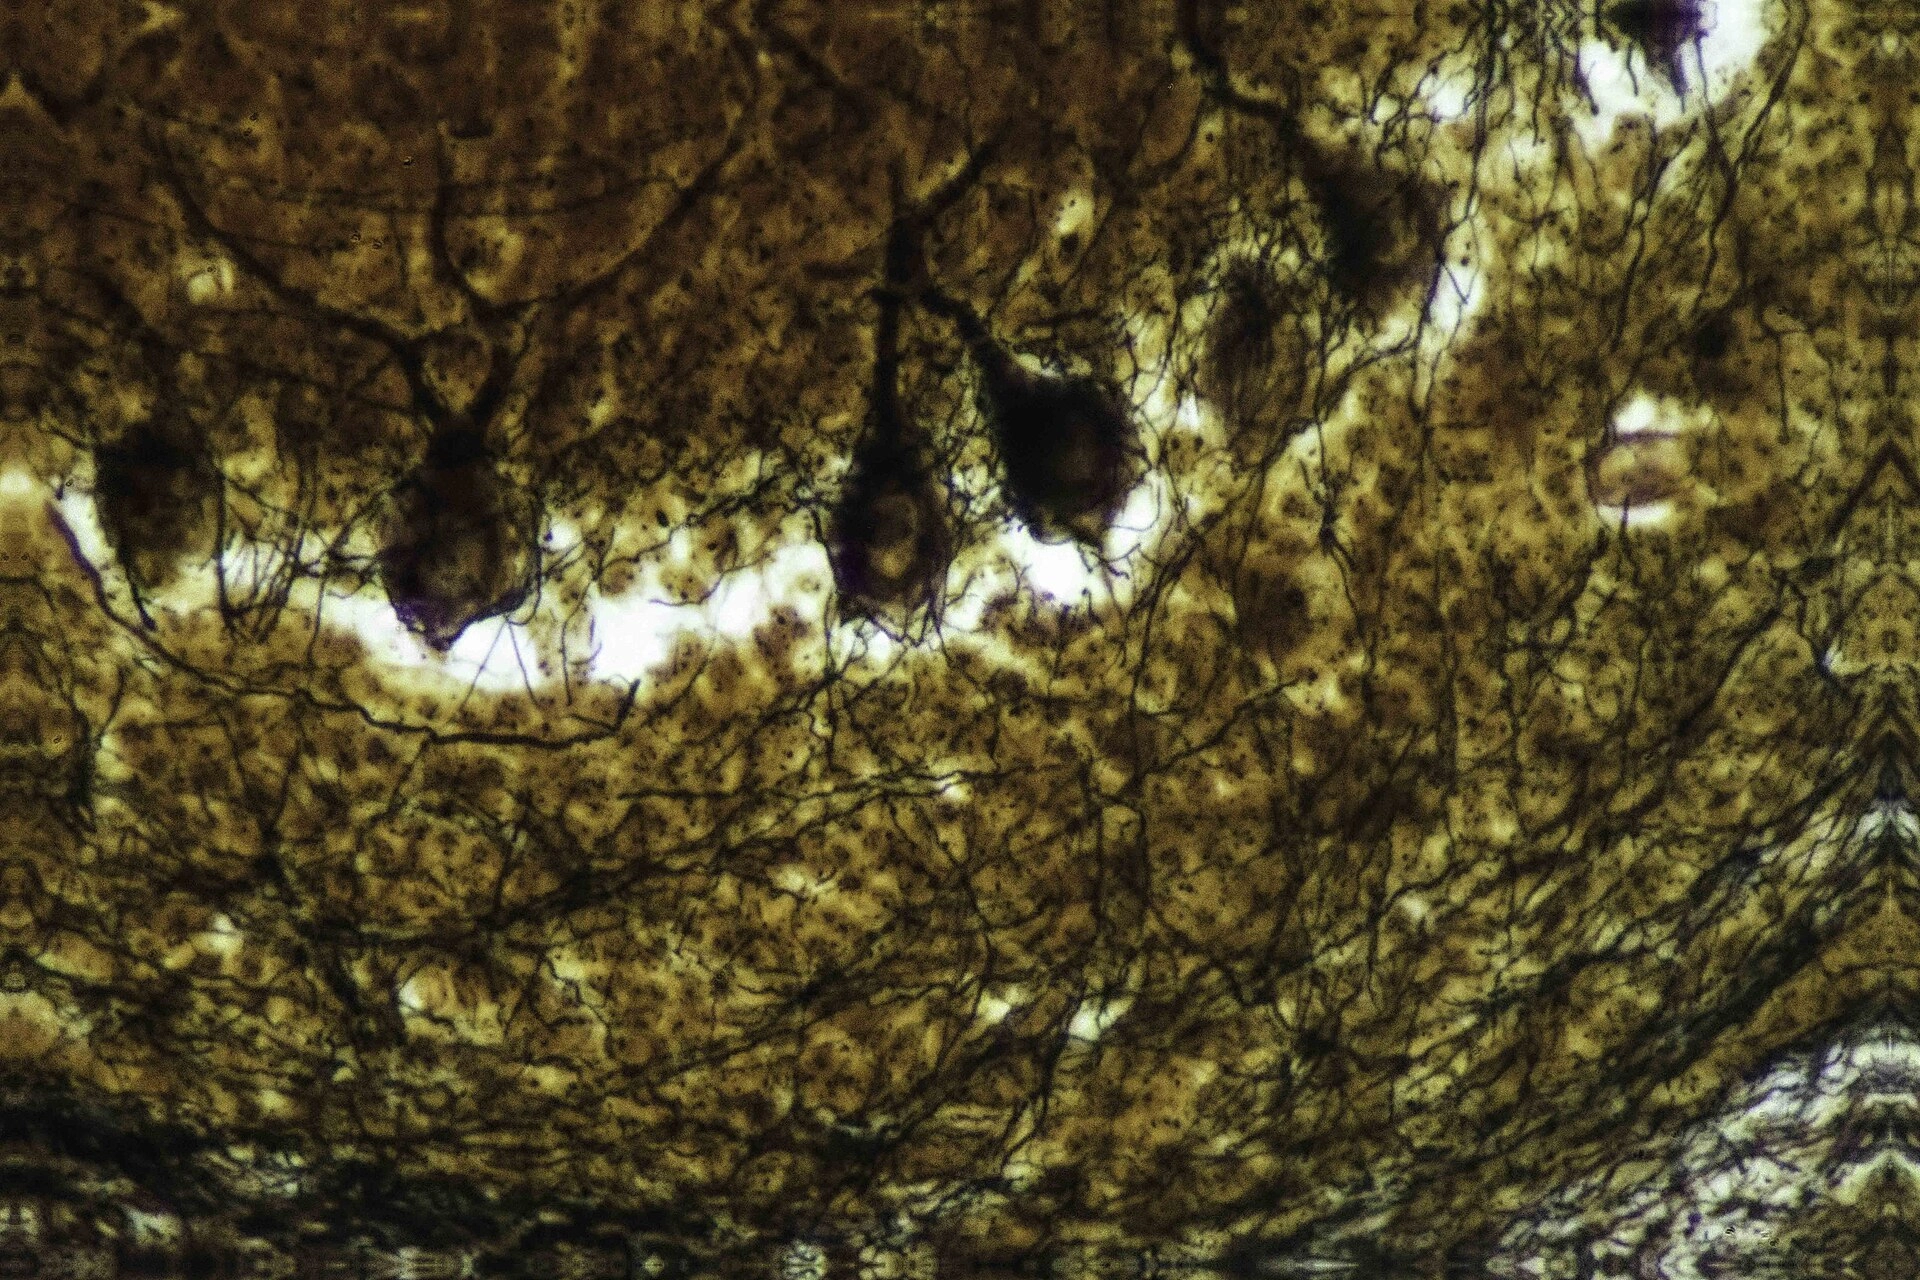
\includegraphics[width=0.75\linewidth]{figures/purkinje-cell.png}
\caption{Purkinje cells as biological reference: parallel integration,
ongoing spontaneous firing, and inhibitory gating of downstream pathways.}
\label{fig:purkinje-cell-diagram}
\end{figure}

This motivates a controller that does more than nearest-neighbor retrieval.
It must combine semantic, episodic, and temporal evidence, then gate what
enters active context, including internally generated candidates. The target
is not maximal storage, but reliable influence control at decision time.

\subsection{Ebbinghaus Forgetting Curve}

The Ebbinghaus forgetting curve captures a practical principle: memory
retention drops without reinforcement \cite{lewandowsky2015ebbinghaus}. For
LLM memory systems, this implies that useful information should gain weight
through reuse, while low-value details should decay automatically.

\begin{figure}[H]
\centering
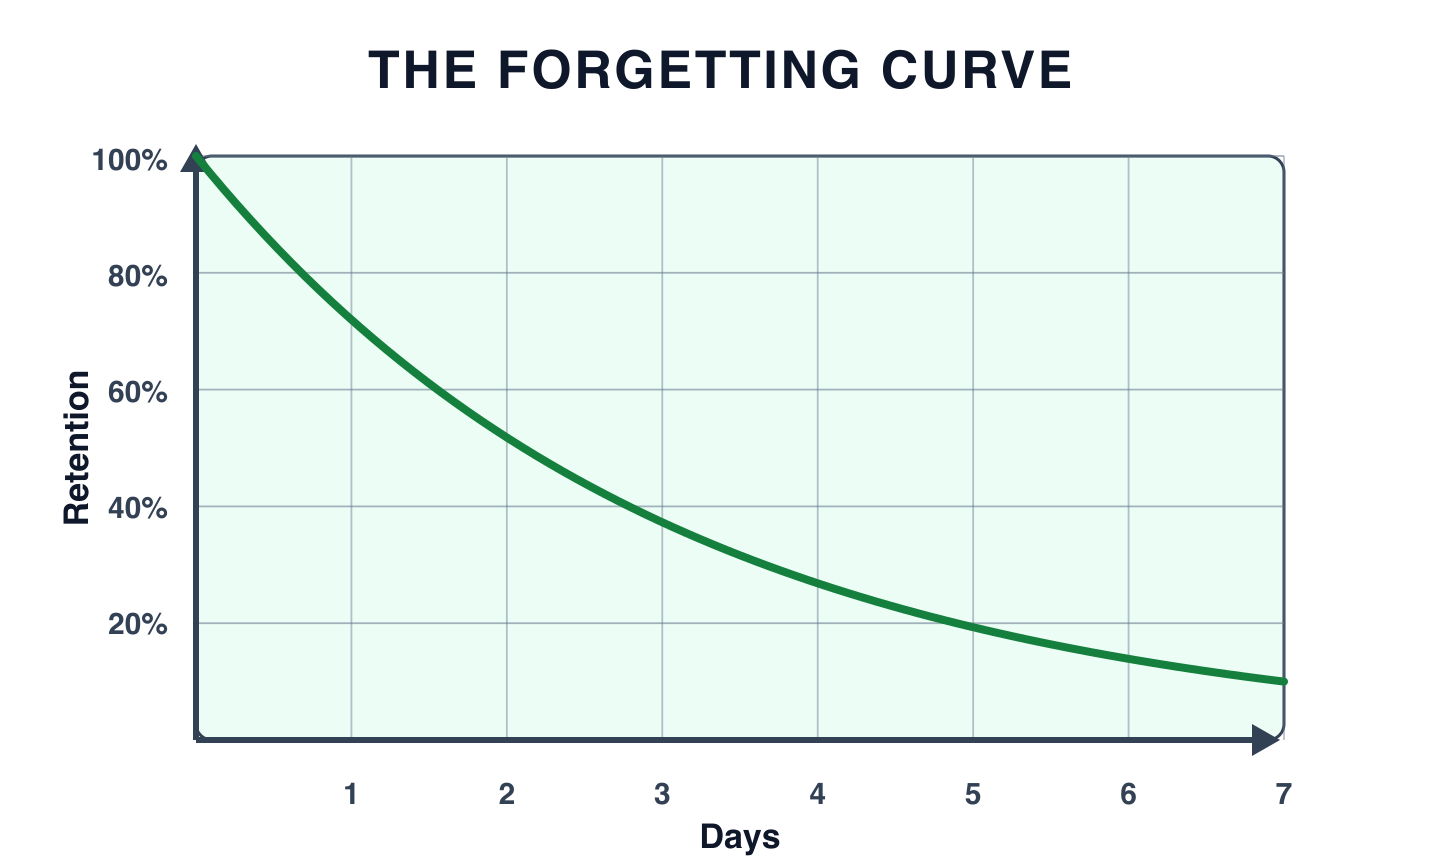
\includegraphics[width=0.75\linewidth]{figures/forgetting-curve.png}
\caption{Ebbinghaus-inspired forgetting dynamics: retention drops rapidly
without reinforcement, motivating selective memory maintenance.}
\label{fig:forgetting-curve}
\end{figure}

This yields a concrete strategy: encode candidate memories at write time, then
update retention from access frequency, recency, and utility. Periodic pruning
and reweighting reduce stale noise while preserving salient patterns.

\subsection{Conscious and Subconscious Processing}

Another useful distinction is conscious versus subconscious processing. The
conscious layer is task-facing and prompt-responsive. The subconscious layer
is continuous and background: it consolidates experience, updates associations,
and reweights salience between explicit tasks. This supports a key design
choice in TinyCortex: recall quality depends on both query-time retrieval and
ongoing maintenance cycles.

\section{Consciousness Loop}

We now describe the core operational mechanism: a recurring four-phase loop
that updates memory and policy state continuously.

In production, most incoming data is initially \textbf{noise}: high-volume,
redundant, and weakly structured. Phase~1 filters and normalizes this stream
before storage. The loop then executes:
\textbf{(1)} ingestion, \textbf{(2)} interval recall and thought synthesis,
\textbf{(3)} action decision, and \textbf{(4)} memory reweighting plus
thought persistence. Over time, this converts raw interaction history into a
compact evolving internal model.

% Source diagram: figures/consciousness-loop.svg (export PNG, e.g.\
% \texttt{rsvg-convert -w 1440 -o figures/consciousness-loop.png figures/consciousness-loop.svg}).
\begin{figure}[H]
\centering
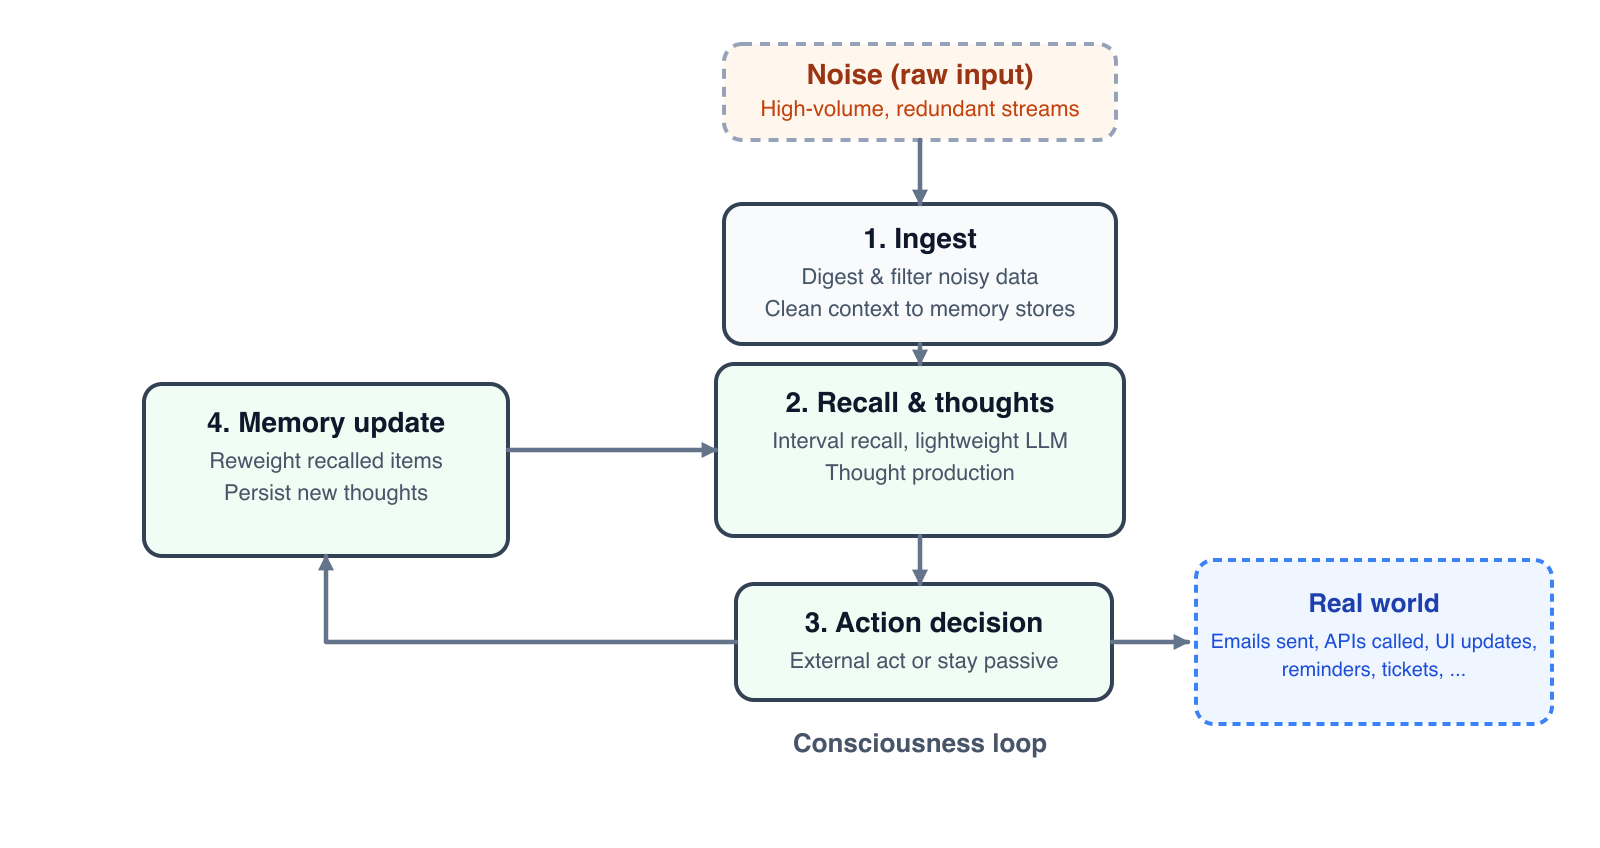
\includegraphics[width=0.98\linewidth]{figures/consciousness-loop.png}
\caption{Control loop: raw \emph{noise} feeds ingest, which filters and
structures data for recall and thought synthesis; action may emit side
effects into the \emph{real world} (email, APIs, UI), while memory
reweighting feeds back into recall---not into ingest or the raw-noise path.}
\label{fig:consciousness-loop}
\end{figure}

\subsection{Phase 1: Large-Scale Contextual Ingestion}

Phase~1 ingests heterogeneous signals that describe entity state and behavior:
emails, direct messages, documents, notes, tickets, logs, and related
artifacts. Inputs are normalized, chunked, and mapped into multiple stores:
semantic vectors, entity-relation graphs, and ordered state-transition events.

This enables later recall from complementary views:
``what is relevant,'' ``what is connected,'' and ``what changed over time.''
Importantly, ingestion is not passive accumulation; early filtering suppresses
repetitive, low-signal, and non-actionable fragments.

\subsection{Phase 2: Interval-Based Recall and Thought Synthesis}

Phase~2 runs on a fixed interval, independent of user prompts. Each cycle
recalls a compact high-salience set using recency, relevance, interaction
frequency, and surprise-weighted signals. Instead of passing large raw context
to a heavy model, the system sends this compact packet to a lightweight LLM.

The objective is \textbf{thought production}, not long-form text generation:
short latent-state updates such as ``new preference inferred,''
``contradiction detected,'' ``follow-up risk,'' or ``candidate next action.''

\subsection{Phase 3: Action Decision}

Phase~3 decides whether to take \textbf{external action} or remain passive.
Given recalled context and synthesized thoughts, a policy checks confidence and
priority thresholds for outbound effects (for example reminders, follow-ups,
or external system updates). If thresholds are not met, the loop continues
with internal updates only.

\subsection{Phase 4: Memory Update and Thought Persistence}

Phase~4 closes the cycle by \textbf{reweighting} recalled memories. Items that
improved the decision are reinforced; items that were unused or misleading are
decayed. Figure~\ref{fig:reinforcement-weights} illustrates this with a toy
graph where one activated path is strengthened while alternatives remain weak.

\begin{figure}[H]
\centering
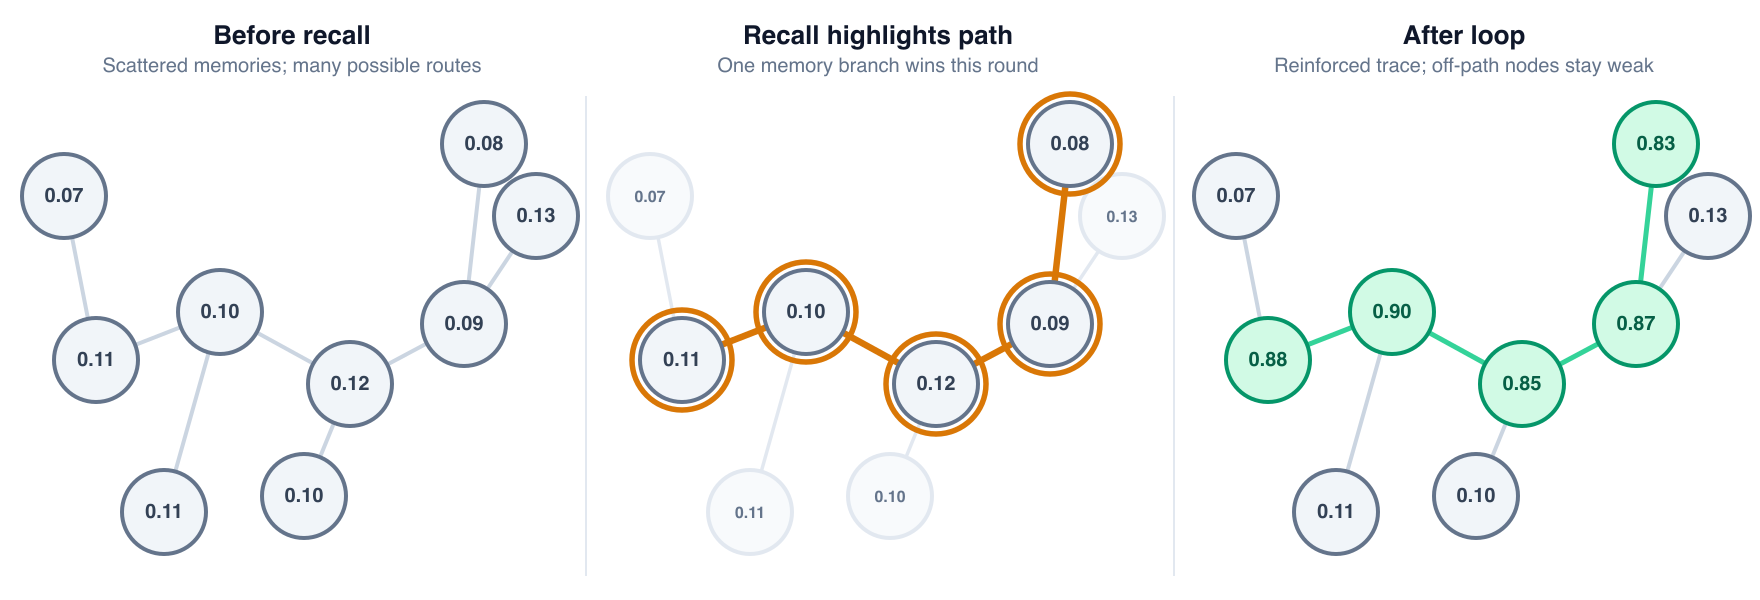
\includegraphics[width=\linewidth]{figures/reinforcement-weights.png}
\caption{Reinforcement of weights in Phase~4 (toy subgraph): before recall,
scattered weak branches; middle, recall selects one path; after
reweighting, only that trace is strongly reinforced.}
\label{fig:reinforcement-weights}
\end{figure}

Thoughts produced in Phase~2 are also \textbf{written back} as durable memory
artifacts, so future cycles can retrieve both source evidence and prior
latent-state summaries. Reweighting plus thought write-back implements
subconscious consolidation between intervals.

\subsection{Why This Loop Matters}

This loop separates expensive context accumulation from cheap continuous
cognition. Periodic recall, lightweight prompting, and explicit write-back
maintain evolving internal state without requiring a heavy model call at every
interaction.

More importantly, this loop creates system-level traits associated with
conscious intelligence: \textbf{feedback} (actions and outcomes alter future
weights), \textbf{learning} (useful patterns are reinforced into latent
state), and \textbf{forgetting} (noise decays unless revalidated). In this
view, TinyCortex is not merely a memory layer; it is a practical control
mechanism for adaptive intelligence growth.

\section{Implementation \& Results}

We implement TinyCortex as a custom memory stack coupled to a lightweight LLM
within the loop above. We then modify the inference layer of an open-source
LLM runtime to consume TinyCortex recall packets and write back thought/memory
updates each cycle.

\begingroup
\setlength{\abovecaptionskip}{6pt}
\setlength{\belowcaptionskip}{0pt}
\begin{figure}[H]
  \centering
  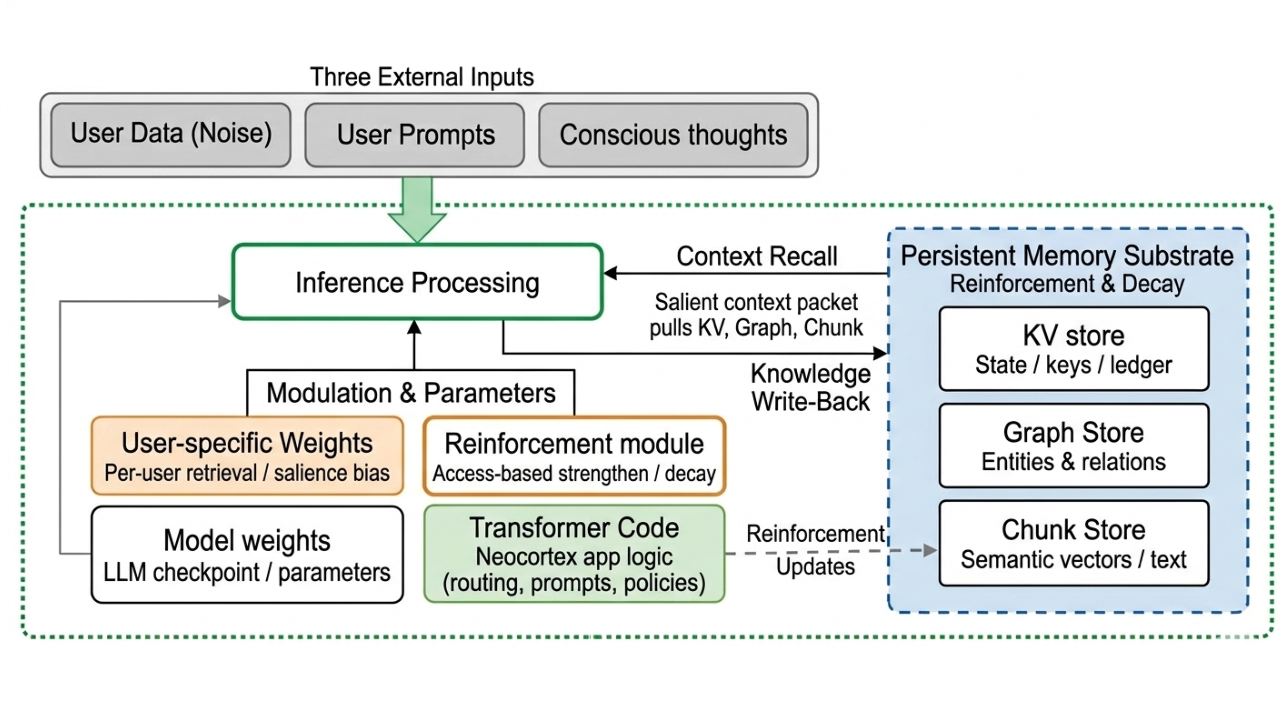
\includegraphics[width=\linewidth,height=0.36\textheight,keepaspectratio]{figures/consciousness-architecture.png}
  \refstepcounter{figure}%
  \label{fig:consciousness-architecture}
\end{figure}
\endgroup

No LLM is required in ingestion or deterministic recall routing. LLM usage is
concentrated in thought synthesis and action decision, which keeps the system
practical under large context volumes.

Evaluation is ongoing across reasoning and memory benchmarks to measure both
decision quality and retrieval/state accuracy.

\subsection{Current Evaluation Status}

This draft reports architecture and loop behavior. We do not claim full
artificial consciousness or benchmark leadership at this stage. The current
evidence is implementation-oriented and qualitative, but it already indicates
improvements in feedback-driven adaptation and learning/forgetting balance.

\subsection{Observed Behavior}

Across long-running internal traces, we observe three recurring effects:
\textbf{(1)} stronger cross-session continuity from explicit state-event
tracking,
\textbf{(2)} lower active-context noise from retention-aware decay, and
\textbf{(3)} better performance on temporal/state queries through ledger-based
routing.

These gains are most visible in mixed tasks where systems must distinguish
``relevant'' from ``currently true.''

\subsection{Limitations and Next Measurement Steps}

Current evidence is primarily qualitative. Formal benchmarking, including
ablations for routing, forgetting, and thought write-back, remains in
progress. The next version will add:
\textbf{(i)} quantitative deltas against baselines,
\textbf{(ii)} latency and token-cost decomposition, and
\textbf{(iii)} error analysis by query type.


\section{Conclusion}

Prior work including Titans/MIRAS, GraphRAG, and MemoryBank demonstrates the
importance of structured memory and retention-aware mechanisms. TinyCortex
extends this direction with an operational conscious-intelligence loop that
integrates ingestion, interval recall, action policy, and write-back
reweighting in one production workflow.

Biological inspiration from the human brain
(Purkinje-style endogenous activity, Ebbinghaus-style decay, and conscious/subconscious separation)
maps to three engineering requirements: selective integration, principled forgetting, and continuous consolidation.

Combined with a strong memory system and an explicit consciousness loop (ingest, recall, act, reinforce), these ingredients yield better intelligence in practice.

\bibliographystyle{unsrt}
\nocite{
  zhong2023memorybank,
  behrouz2025titans,
  behrouz2025allconnected,
  fountas2024emllm,
  jimenez2024hipporag,
  edge2024graphrag,
  wu2025survey,
  lewandowsky2015ebbinghaus,
  clewett2024predictions,
  kim2024predictionerror
}
\bibliography{references}

\end{document}
